% Set the Page Layout
\documentclass[12pt]{article}
\usepackage[inner = 2.0cm, outer = 2.0cm, top = 2.0cm, bottom = 2.0cm]{geometry}
\usepackage{biblatex}
\usepackage{graphicx}
% Package to write pseudo-codes
\usepackage{algorithm}



% Don't Remove the 'end' at the end of the algorithm
\usepackage{algpseudocode}

% Manually remove the 'end' for some sections
\algtext*{EndIf}
\algtext*{EndFor}
\algtext*{EndWhile}

% Define Left Justified Comments
\algnewcommand{\LeftComment}[1]{\Statex \(\triangleright\) #1}

% Remove the Numbering of the Algorithm
\usepackage{caption}
\DeclareCaptionLabelFormat{algnonumber}{Algorithm}
\captionsetup[algorithm]{labelformat = algnonumber}

% Define the command for a boldface instructions
\newcommand{\Is}{\textbf{ is }}
\newcommand{\To}{\textbf{ to }}
\newcommand{\Downto}{\textbf{ downto }}
\newcommand{\Or}{\textbf{ or }}
\newcommand{\And}{\textbf{ and }}
% Use them inside Math-Mode (Hence the space!)

\begin{document}

\begin{algorithm}

  \caption{Topological sort using Kahn's algorithm  \cite{1}}
  
  \begin{algorithmic}[1]
    \Statex
        \State $L \gets Empty\ list\ that\ will\ contain\ the\ sorted\ elements $
        \State $S \gets Set\ of\ all\ nodes\ with\ no\ incoming\ edge\ $
        \State $inDegree \gets Vector\ where\ inDegree[n]\ is\ the\ number\ of\ incoming\ edge\ of\ the\ node\ n$
        \ForAll{$node\ n\ in\ the\ graph\ $}
            \ForAll{$node\ m\ with\ an\ edge\ e\ from\ n\ to\ m$}
                \State $inDegree[m]++\  (number\ of\ incoming\ edges\ of\ the\ node\ m) $
            \EndFor
        \EndFor
        
        \ForAll{$node\ n\ in\ the\ graph\ $}
            \If{$inDegree[n]\ == 0$}
                \State $ add\ n\ to\ S $
                \EndIf
        \EndFor
        
        
        \While {$ S\ is\ non\ empty\  $}
            \State $remove\ a\ node\ n\ from\ S\ $
            \State $add\ n\ to\ tail\ of\ L\ $
            \ForAll{$node\ m\ with\ an\ edge\ e\ from\ n\ to\ m $}
                 \State $inDegree[m]--\  (number\ of\ incoming\ edges\ of\ the\ node\ m) $
                \If{$ m\ has\ no\ other\ incoming\ edges\ (inDegree\ ==\ 0)$}
                    \State $insert\ m\ into\ S$
                \EndIf
            \EndFor
        \EndWhile
        \If{$ grap\ has\ no\ edges$}
            \State $return\ error\  \ \ \ (graph\ has\ at\ least\ one\ cycle)$
        \Else
        \State $return\ L\  \ \ \ (a\ topologically\ sorted\ order)$
        \EndIf
  \end{algorithmic}
 
\end{algorithm}

Example:
\begin{figure}[H]
\centering
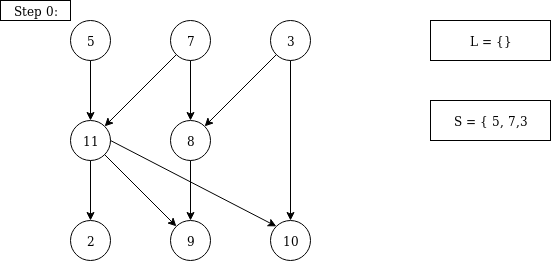
\includegraphics[width=100mm]{KahnAlgoStep1.png}
\caption{init state}
\end{figure}

\begin{figure}[H]
\centering
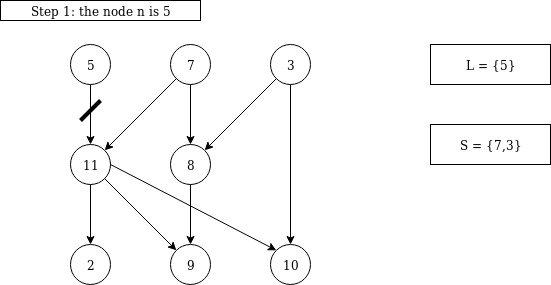
\includegraphics[width=100mm]{KahnAlgoStep2.png}
\caption{state 1}
\end{figure}

\begin{figure}[H]
\centering
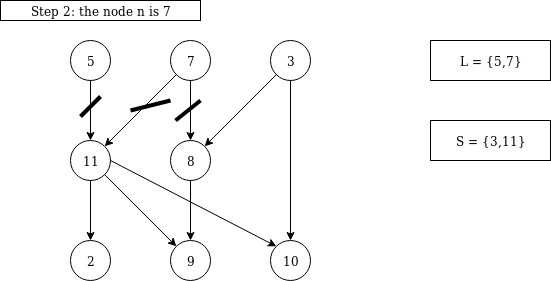
\includegraphics[width=100mm]{KahnAlgoStep3.png}
\caption{state 2}
\end{figure}

\begin{figure}[H]
\centering
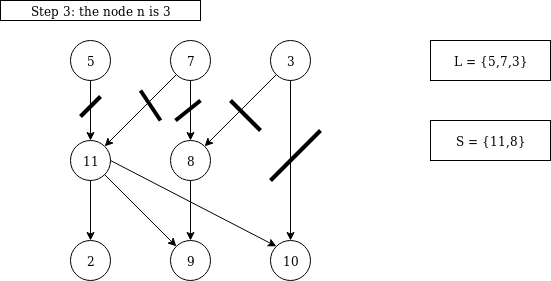
\includegraphics[width=100mm]{KahnAlgoStep4.png}
\caption{state 3}
\end{figure}
    
    
    \begin{figure}[H]
\centering
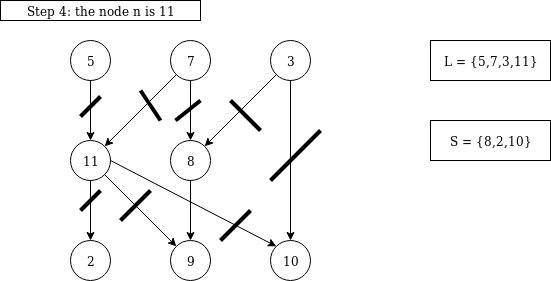
\includegraphics[width=100mm]{KahnAlgoStep5.png}
\caption{state 4 }
\end{figure}

\begin{figure}[H]
\centering
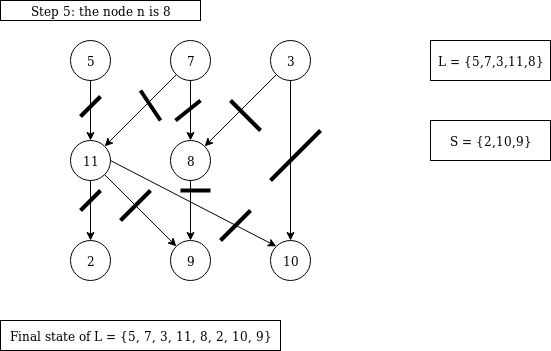
\includegraphics[width=100mm]{KahnAlgoStep6.png}
\caption{state 5}
\end{figure}
    
    


\begin{thebibliography}{1}
\bibitem{wikipedia} 
Topological sort: Kahn's algorithm
\\\texttt{$https://en.wikipedia.org/wiki/Topological\_sorting\#Kahn's\_algorithm$}

\end{thebibliography}



\end{document}